\subsubsection{E/S}

\paragraph{Question 1} (E/S). Énoncer les propriétés importantes des "interruptions précises" et de leur intérêt pour les concepteurs des systèmes d'exploitation.
\color{reponse}
\begin{itemize}
	\item Ce sont des interruptions qui garantissent que l'état des registres est cohérent après son exécution par 4 propriétés:
		\begin{enumerate}
			\item Le PC (program counter) est sauvé dans un endroit connu.
			\item Toutes les instructions précédant l'instruction pointée par PC ont été totalement exécutée.
			\item Aucune instruction après n'a été exécutée.
			\item L'état de l'instruction pointée par PC est connu.
		\end{enumerate}
	Ces conditions peuvent paraître évidentes, mais on doit y faire attention, particulièrement dans le cas de pipelines où des instructions pourraient être partiellement exécutées, ou dans le cas d'instructions d'entrées sorties dont le principe est basé sur des effets de bords. Certains processeurs comme les x86 actuels réordonnent aussi les instructions pendant l'exécution, il faut donc en tenir compte. (Infos en plus: \url{http://lwn.net/images/pdf/LDD3/ch09.pdf})
\end{itemize}
\color{black}



\paragraph{Question 2} (E/S). À l'aide d'un schéma expliquer l'accès direct à la mémoire (DMA, \textit{Direct Memory Access}). En particulier décrivez les 4 étapes vues au cours.
\color{reponse}
\begin{center}
	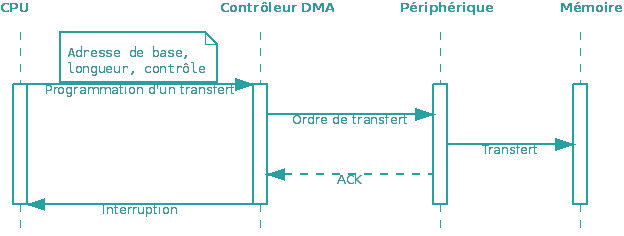
\includegraphics[scale=0.5]{2.questions_et_reponses/2.oral/4.entree_et_sortie/ESQ3.png}
\end{center}
\begin{enumerate}
	\item Le CPU programme le contrôleur DMA: il initialise un registre avec l'adresse de base, un autre avec la longueur du transfert et des registres de contrôle (direction du transfert (read/write) par exemple). 
	\item Le contrôleur DMA envoie le message au périphérique (pendant ce temps le CPU fait autre chose).
	\item Le périphérique effectue le transfert vers ou depuis la mémoire et le signale au contrôleur DMA quand il a fini.
	\item Le contrôleur DMA déclenche une interruption pour signaler que la transaction est finie.
\end{enumerate}
\color{black}



\paragraph{Question 3} (E/S). Pourquoi les fichiers de sortie de l'imprimante sont-ils normalement "spoulés" sur disque avant d'être imprimés ?
\color{reponse}
\begin{itemize}
	\item Le service spouleur d'impression permet de charger en mémoire les travaux d'impression pour une impression ultérieure, c'est-à-dire comme une imprimante ne peut imprimer qu'un fichier à la fois on va le mettre dans la file d'attente afin de ne pas bloquer l'accès au fichier lors de l'impression. Quand l'imprimante à fini avec un fichier, c'est le fichier suivant dans le spouleur qui est envoyé automatiquement à l'imprimante.
	\\Si des fichiers restent bloqués dans le spouleur c'est que l'imprimante à un problème (plus papier, plus d'encre,...) ou que l'impression du fichier a été suspendu. Sur un ordinateur personnel, on exploite rarement le spoulage d'entrée mais en revanche, on utilise le spoulage de sortie.
\end{itemize}
\color{black}



\paragraph{Question 4} (E/S). Supposez qu'un ordinateur puisse lire ou écrire un mot mémoire en 10 ns. Supposez également que, lorsqu'une interruption se produit, les 32 registres du processeur, plus le compteur ordinal et le mot d'état du programme, soient placés sur la pile. Quel est le nombre maximal d'interruptions par seconde que cet ordinateur peut traiter ?
\color{reponse}
\begin{itemize}
	\item Il faut placer 34 mots sur la pile pour chaque interruption. Le retour de l'interruption nécessite l'extraction de 34 mots de la pile. Cette seule surcharge représente 680 ns. Ainsi, le nombre maximum d'interruptions par seconde est de 1,47 million, sans effectuer le moindre travail pour les interruptions.
\end{itemize}
\color{black}



\paragraph{Question 5} (E/S). De nombreuses versions d'UNIX utilisent un entier 32 bits non signé pour suivre l'heure sous la forme d'un nombre de secondes écoulées depuis l'origine du temps. Quand ces systèmes vont-ils boucler (année et mois) ? Pensez-vous que cela se produira réellement ?
\color{reponse}
\begin{itemize}
	\item Le nombre de secondes d'une année moyenne est de $365,25*24*3600=31.557.600$. Le compteur boucle après $2^{32}$ secondes à partir du $1^{er}$ janvier 1970. La valeur de $2^{32}/31.557.600$ donne 136,1 ans. La boucle se produira donc à 2.106,1 soit début février 2106. D'ici là, tous les ordinateurs utiliseront au moins 64 bits, donc cela ne se produira pas.
\end{itemize}
\color{black}



\paragraph{Question 6} (E/S). Une page de texte imprimée classique contient 50 lignes et 80 caractères chacune. Imaginez qu'une imprimante donnée puisse imprimer 6 pages/minutes et que le temps d'écrire un caractère dans le registre de sortie de l'imprimante soit si court qu'il puisse être ignorée. Est-il logique d'exécuter cette impression avec des E/S pilotées par les interruptions si chaque caractère imprimé demande une interruption qui prend 50 µs en tout ?
\color{reponse}
\begin{itemize}
	\item 
\end{itemize}
\color{black}